% ChapterPub1

%\label{ChapterPub1} % For referencing the chapter elsewhere, use \ref{ChapterPub1} 

%\lhead{Chapter 2. \emph{Methods}} % This is for the header on each page - perhaps a shortened title

\pagestyle{empty}

\addtocontents{toc}{\cftpagenumbersoff{chapter}}



\begin{center}
\setcounter{chapter}{0}
\chapter{Wolfisberg et al., Journal of Virology, Submitted November 2015}

\bigskip
\bigskip
\bigskip
\bigskip

\LARGE{\textbf{Late maturation steps in the nucleus preceding prelytic active egress of
progeny parvovirus.}}

\bigskip
\bigskip
\bigskip

Raphael Wolfisberg, Christoph Kempf and Carlos Ros
\end{center}

\phantomsection\addcontentsline{toc}{section}{Late Maturation Steps in the Nucleus Preceding Prelytic Active Egress of Progeny Parvovirus.}



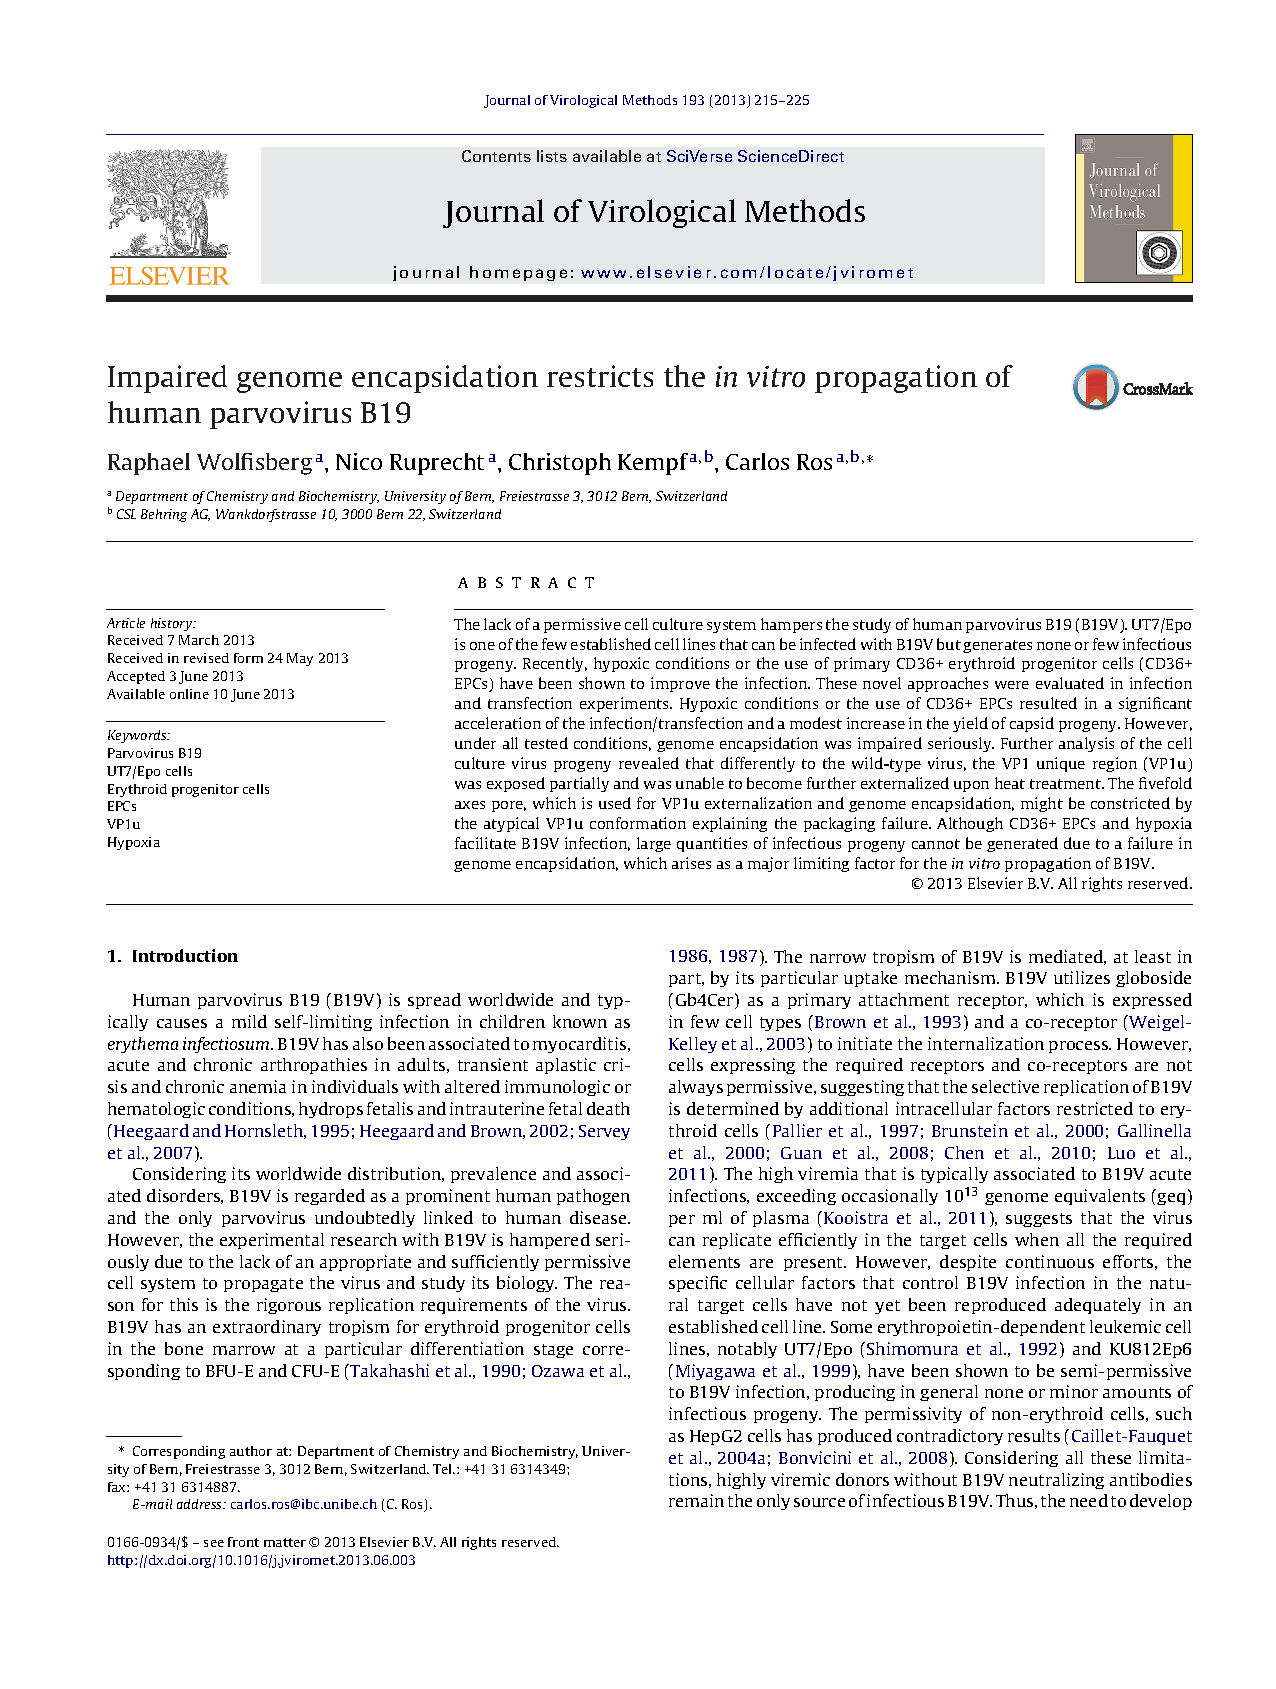
\includepdf[pagecommand=\thispagestyle{empty}, pages={1-11}, scale=0.9]{../pdfdocuments/b19vpaper}


\setcounter{chapter}{9}
